%!TEX root = ../thesis.tex
%*******************************************************************************
%*********************************** First Chapter *****************************
%*******************************************************************************

\chapter{Further studies: Do the Optimization and find more underlying physics}  %Title of the First Chapter

\graphicspath{{Chapter4/}}


%********************************** %First Section  **************************************
\setlength{\epigraphwidth}{0.6\textwidth}
\epigraph{“I first heard of this when Fowler was explaining it to one of Rutherford’s closest collaborators, who said ‘very interesting’ in a tone which implied that he was not interested at all. Neither was I.”}
{\textit{Nevil Mott, recollecting the glorious moment he first learned of the difference between metals and insulators.}}
\section[The Bayesian Optimization on ITC]{Designing Nanostructures for Phonon Transport via Bayesian Optimization}
\textit{Thermal boundary resistance (TBR) is a key property for the thermal management of high power
micro- and opto-electronic devices and for the development of high efficiency thermal barrier coatings
and thermoelectric materials. Prediction of TBR is important for guiding the discovery of interfaces
with very low or very high TBR. Based on our study on phonon transmittance between III-V semi-conductors interfaces, we report the prediction of TBR by the machine learning method, our main method is the Bayesian Optimization which also includes the Gussian process regression. The application of this method has been proved efficient in work\cite{ueno2016combo}, and our work is also based on this work and the open code available at \url{https://github.com/tsudalab/combo}. }\\
\textit{We demonstrate optimization of thermal conductance across nanostructures by developing a method combining atomistic Green's function and Baysian optimization. With an aim to minimize and maximize the interfacial thermal conductance(ITC) across four types of III-V semi-conductors(AlP,AlAs,GaP,GaAs) superlattices, the method identifies the optimal structures from calculations of only a few percent of the entire candidates(over $4^6$ structures). The obtained optimal interfacial structures are nonintutive and impacting. The work shows the effectiveness and advantages of material informatics in designing nanostructures to control heat conduction, which can also be extended to other nanostructures and properties\cite{ju2017designing}.}
\subsection{Introduction}
During the past decade, informatics has been successfully applied in many aspects\cite{rajan2015materials,agrawal2016perspective}, namely the integration of
material property calculations or measurements and informatics to accelerate the material discovery and design. In the field of heat transfer, materials informatics has been applied to search for thermalelectric material with low thermal conductivity\cite{carrete2014finding}. However, the nanostructure optimization for thermal transport, especially in multi-structures is still in its infancy. In this work, we use the Bayesian optimization methods based on our former atomistic Green's function(AGF) method to identify the interficial strutures that realize maximum and minimum ITC.
\subsection{Methodolody}
%%%%%%%%%%%%%%%%%%%%%%%%%%%%%%%%%%%%%%%%%%%%%%%%%%%5
\begin{figure}

\centering
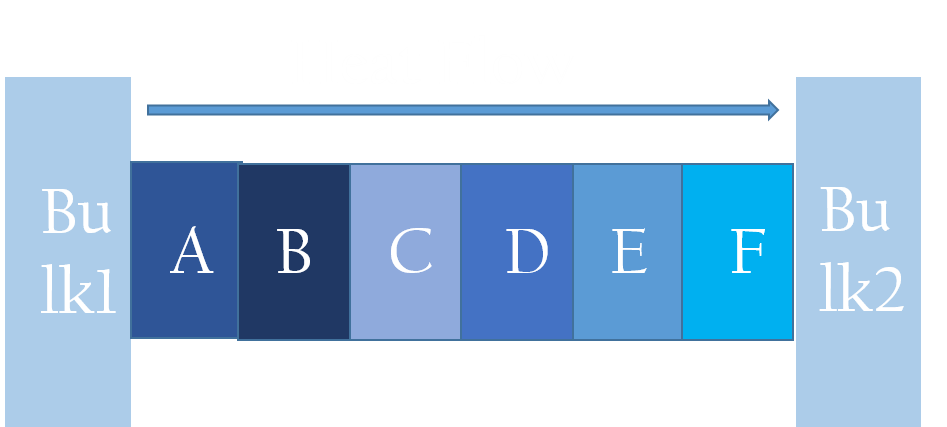
\includegraphics[width=0.5\textwidth]{device.png}
\caption{The illustration of the structure we study}
\label{fig:agfdevice}
\end{figure}
\begin{figure}
\centering
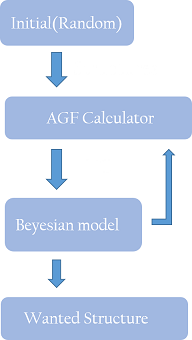
\includegraphics[height=8cm]{map.png}
\caption{Schematics of the materials informatics method combing the atomistic Green function (AGF) and Bayesian optimization}
\label{fig:agfmap}

\end{figure}
%%%%%%%%%%%%%%%%%%%%%%%%%%%%%%%%%%%%%%%%%%%%%%%%%%%%%
We explain the method by taking a problem to design the superlattice interfacial strcuture to tune the heat conduction across the interface between AlP, AlAs, GaP and GaAs. As illustrated in Fig(\ref{fig:agfdevice}), the system consists of an interfacial region between two materials A(AlP) and B(AlP) with infinite thickness. For the convinience of calculation, the lattice mismatch between these four materials is ignored because this effect has been included in our former study in Chapter 3.
The interfacial structure is divided into six parts, each of which can consist of AlP,AlAs,GaP or GaAs, and the optimization problem is how to arrange the Si and Ge atoms to obtain the largest and the smallest ITC.\\
\indent Four basic elements are required when conducting
material informatics: the descriptor, evaluator, calculator,
and optimization method. The descriptors are used to
describe the possible structure candidates considered during the optimization. 
In this study, we use several ints to
describe the state of each atom: “1”,“2”,“3” and “4” represent the
AlP,AlAs,GaP and GaAs atom, respectively. As for the evaluator, the value
of ITC is chosen to quantitatively evaluate the performance
of each configuration.\\
\indent Because we have given the explicit form of AGF method in form Chapter, now we just give a breif introduction of the Bayesian Optimization method.Actually, we are interested in solving that a problem:
\begin{equation*}
x^{*}=arg min_x f(x)
\end{equation*}
Under the constraints that
\begin{itemize}
	\item $f$ is a black box for which no closed form is know(nor its gradients)
	\item $f$ is expensive to evaluate
	\item And evaluation of $y=f(x)$ may be noisy
\end{itemize}
Under these conditions, it is quite nice to employ the Bayesian optimization method. Below is a standard Bayesian optimization loop\cite{snoek2012practical}:\\
For $t=1:T$:
\begin{enumerate}
	\item Given observations $(x_i,y_i=f(x_i))$ for $i=1:t$, build a probabilistic model for the objective $f$. Itegrate out all possible true functions, using Gaussian process regression\cite{rasmussen2006gaussian}. 
	\item Optimize a cheap acquisition/utility function $\mu$ based on the posterior distribution for sampling the next point
	\begin{equation*}
	x_{t+1}=arg min_x \mu(x)
	\end{equation*}
	Exploit uncertainty to balance exploration against exploitation.
	\item Sample the next observation $y_{t+1}$ at $x_{t+1}$
\end{enumerate}
Then comes the core of this method: Acquisition functions\cite{brochu2010tutorial}.Acquisition functions $\mu(x)$ specify which sample $x$ should be tried next
\begin{itemize}
	\item Expected improvement(default): $-EI(x)=-\mathbb{E}[f(x)-f(x^{+}_t)]$
	\item Lower confidence bound: $LCB(x)=\mu_{GB}(x)+\kappa \sigma_{GP}(x)$
	\item Probaility of improvement: $-PI(x)=-P(f(x) \geq f(x^{+}_t)+\kappa)$
\end{itemize}
where $x^{+}_t$ is the best point observed so far.\\
\indent In our work, we emplot the open-source Bayesian optimization library $\mathcal{COMBO}$\cite{ueno2016combo} to perform the optimization process. Bayesian optimization is an experimental design algorithm based on machine learning\cite{jones2001taxonomy}. As shown in Fig(\ref{fig:agfmap}), suppose that ITCs of $n$ candidates are initially calculated, and we are to choose the next one to calculate. A Bayesian regressio function is learned from $n$ pairs of descriptors and ITCs(training examples). For each of teh remaining candidates, a predictive distribution of ITCs is estimated. The best candidate is choosen based on the criterion of expected improvement\cite{jones2001taxonomy}.Finally, ITC is calculated for the chosen candidate, and it is added to the training examples. By repeating this procedure, the calculation of ITCs is scheduled optimally, and the best candidate can be found quickly.\\
\indent As the prediction model, we exploy a Bayesian linear regression model combine with a random feature map,
\begin{equation}
y=w^{T}\psi(x) +\epsilon
\end{equation}
where $x$ is a d-dimensional vector corresponding to a candidate, $w$ is a D-dimensional weight vector, and $\epsilon$ is the noise subject to normal distribution with mean 0 and variance $\sigma$. The random feature map is chosen so that the inner product corresponds to the Gaussian kernel\cite{rahimi2008random}:
\begin{equation}
\psi(x)^T\psi(x^{'})=exp(-\frac{|x-x^{'}|^2}{\eta^2})
\end{equation}
\indent The performance of the model depends on hyperparameters $\sigma$ and $\eta$. In $\mathcal{COMBO}$, they are initialized according to a heuristic procedure bu Yang $et al.$\cite{yang2015carte}. 
\subsection{Reuslts and Discussion}
In our calculation, the predicted struture with maximum ITC comes to convergence within calculations less than 200 structures, which is only $4.9\%$ of the total number of candidates(4096). In Fig(\ref{fig:maxITC}), we also calculate the structures with no interface to compare with the optimazed structures. It can be clearly seen that almost in all frequencies, the aimed structure(412314) has very low transmittance. For phonon energy in the central region(0.015eV-0.025eV), the wave-length of phonons is almost the same as the length of unit cell so that the transmissions of different strutures can be very similar. On the other hand, in other regions, the transmission function strongly depends on the strcuture.
\begin{figure}
\centering
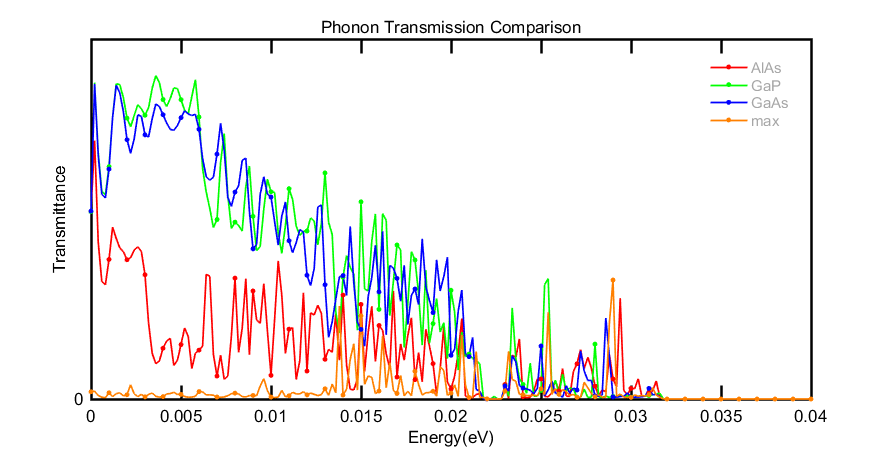
\includegraphics[width=0.8\textwidth]{max.png}
\caption{The illustration of the structure we study}
\label{fig:maxITC}
\end{figure}\\
\indent Now that the optimal struture is identified, we can move on  to look into the mechanisms behind the big ITC. And this is actually the goal of the next work, and for this topic here, there are mainly below ways to discuss:
\begin{enumerate}
	\item The first
obvious attempt is to see it from the view of phonon
dispersion relations and phonon density of states (DOS), as
is broadly done to discuss phonon interference.
	\item Then to gain a deeper understanding of the physics of
phonon transport in the optimized structure, we can look into
the role of phonon coherence, which can cause constructive
and destructive interferences.
\end{enumerate}
\subsection{Conclusions}
In conclusion, we identify the III-V semi-conductors composite interfacial structures that maximize the ITC across two contacts by the developed framework combining the atomistic Green function and Bayesian optimization methods.The optimal structures are obtained
by calculating only a few percent of the total candidate
structures, considerably saving computational resources. And this work not only gives a practical example to design the thermal nanostructures with desired thermal properties(i.e. ITC), but also leaves us an entrance to further study on the physics behind the data.\\

\setlength{\epigraphwidth}{0.6\textwidth}
\epigraph{“The work using machine learning tool such as Bayesian optimization is quite great, but when you get the final result you still don't know why the result should be like this... You know, regression, may data back to Newton's age, but you can use this to discover real science.”}
{\textit{Junichiro Shiomi(Professor, Univeristy of Tokyo)}}
\section[Figure out the physics]{Study on the factors affecting the ITC and Phonon tramsmittance}

\subsection{Mechanism behind the phonon interface transmittance}
As we have calculated and given primary dicussion in former chapter, we gain the phonon transmittance of total combinations of III-V semi-conductors using AGF method. And we also further use the Bayesian optimization method to get the desired strusture with maximum(or minumum) ITC, our next work will focus on the physcis behing these data, namely:
\begin{itemize}
	\item Find out the factors that affect the transmittance and also the way how they take effect. Then try to establish the new model not just following the old AMM or DMM pattern.
	\item Based on the former work, find out a predictor model to derive the desired structure by the knowledge of physics.
\end{itemize}
\subsection{Regression Analysis}
Actually, there have been several attempts on that issue these years, and the most recent one is the paper\cite{zhan2017prediction} published on Nature Scientific Report in June, 2017. In this work, they combine the past data gained from many past works and try to find out a model to predict the TBR(thermal boundary
resistance). As shown in Fig(\ref{fig:TBR}),the descriptors used for the AMM and DMM predictions are temperature, density, speed of sound (longitudinal and transverse), and unit cell volume, which we defne as “AMM and DMM descriptors”. However, they didn't 'jump out' the famework of AMM and DMM and they only consider the bulk properties so that their work is far from reaching the true physics behind this issue. 
\begin{figure}
\centering
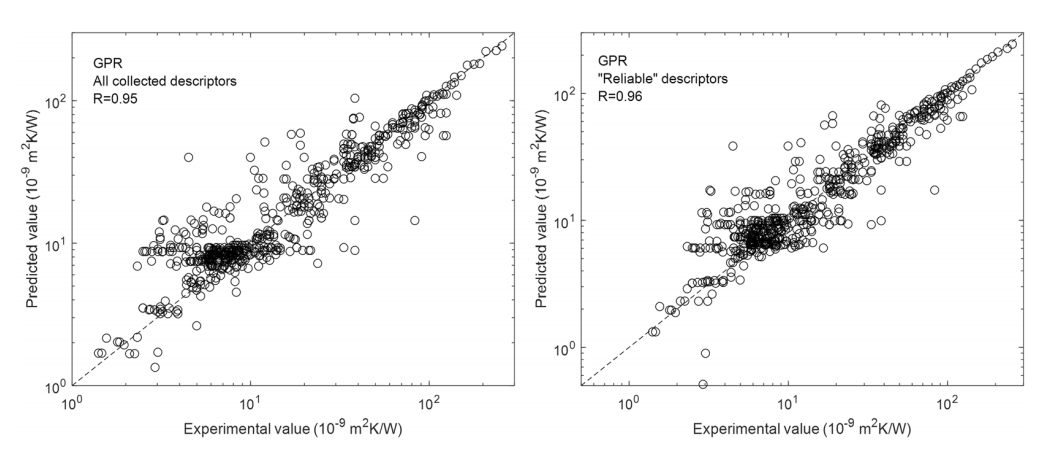
\includegraphics[width=0.8\textwidth]{TBR.png}
\caption{Correlation between the experimental values and the values predicted by the GPR model using the
“reliable” descriptors and all collected descriptors\cite{zhan2017prediction}.}
\label{fig:TBR}
\end{figure}\\
\indent Actually, motivated by a recent work\cite{hua2017slip} on Slip Boundary Conditions in Ballistic–Diffusive Heat Transport, the MFP of phonon is thought to play an important role in phonon interface transmittance. Now we have stepped forward to consider more factors based on derivation of BTE or other experiments to do the regression, and this is the heart of the later work.\\

\textbf{My code of the AGF method and the Bayesian optimization is available at \url{https://github.com/chieko-feiyuxiao/Oric}}